\documentclass{csri08}

% PACKAGES ---------------------------------------------------------------
\usepackage{amsfonts,amsmath,graphicx,subfigure,verbatim}
% ADD YOUR OWN PACKAGES HERE ---------------------------------------------
%\usepackage{someotherpackage}
\usepackage{color,url}

% DEFINITIONS ------------------------------------------------------------
% ADD YOUR OWN DEFINITIONS HERE ------------------------------------------
% BE SURE TO PREFACE LABEL WITH YOUR OWN INITIALS (SSS in this example) --
\definecolor{Red}{rgb}{1,0,0}
\definecolor{IanBlue}{rgb}{0,0,1}
\newcommand{\JJH}[1]{\textcolor{Red}{#1}}
\newcommand{\IK}[1]{\textcolor{IanBlue}{#1}}

\newcommand{\IKcompfont}[1]{{\tt#1}}

% This controls the table-of-contents entry in the proceedings. Edit it
% to include your article title followed by the authors' names, as shown.
\addcontentsline{toc}{chapter}{
Overview and Performance Analysis of the Epetra/OSKI matrix class interface in Trilinos
{\em I.K.\ Student and J.H.\ Mentor}}

\pagestyle{myheadings}

\thispagestyle{plain}

% This gives the running head. Usually you list a shortened version of
% your article title (unless it's already very short) along with
% the author's names, as shown.
\markboth{
Overview and Performance Analysis of the Epetra/OSKI matrix class interface in Trilinos
}{I.K.\ Student and J.H.\ Mentor}

% Put your article title in here
%\title{Epetra OSKI Implementation}
\title{
Overview and Performance Analysis of the Epetra/OSKI matrix class in Trilinos
}

% List each author, their affiliation, and their e-mail address, as shown.
\author{I. Karlin\ Student\thanks{University of Colorado, Boulder, Ian.Karlin@colorado.edu} \and J. Hu\ Mentor\thanks{Sandia National Laboratories,
jhu@sandia.gov}}

\begin{document}

\maketitle

% Include your abstract here.
\begin{abstract}
In this paper, we describe a new matrix class in Epetra that gives a Trilinos application access to the Optimized Sparse Kernel
Interface (OSKI) package.  Epetra is the core basic linear algebra package within Trilinos, Sandia's
numerical algorithms framework.
We give an overview of OSKI and the new Epetra class design.
We also present numerical results that compare performance of equivalent OSKI and Epetra kernels in serial
and in parallel.  Finally, we discuss potential impact of OSKI on applications that currently use
Trilinos.
%Jonathan's draft:
%At Sandia, the repeated parallel solution of linear systems is a critical part of
%many computer simulations.
%Sandia's Trilinos project provides high performance numerical solution methods,
%many of which depend on sparse linear algebra operations, such as matrix vector
%multiplication.  Such operations are provided by the Epetra library within Trilinos.
%Hence, the speed of Epetra kernels can have a large impact on many scientific simulations.
%In this paper, we discuss our implementation of an Epetra matrix class that leverages
%the Optimized Sparse Kernel Interface (OSKI).
%The OSKI project provides many optimized sparse matrix-vector kernels.  By making these
%kernels available in Epetra, we enable application that depend on Trilinos
%to benefit from OSKI's tuned stock kernels and runtime tuning capabilities.
\end{abstract}

\section{Introduction} \label{IK:sec:intro}
%%%%%%%%%%%%%%%%%%%%%%%%%%%%%%%%%%%%%%%%%%%%%%%%%%%%%%%%
%
% Copyright (c) 2003-2012 by University of Queensland
% Earth Systems Science Computational Center (ESSCC)
% http://www.uq.edu.au/esscc
%
% Primary Business: Queensland, Australia
% Licensed under the Open Software License version 3.0
% http://www.opensource.org/licenses/osl-3.0.php
%
%%%%%%%%%%%%%%%%%%%%%%%%%%%%%%%%%%%%%%%%%%%%%%%%%%%%%%%%

\chapter{Introduction}
This document describes how to install \emph{esys-Escript}\footnote{For the rest of the document we will drop the \emph{esys-}} on your computer.
To learn how to use \esfinley please see the Cookbook, User's guide or the API documentation.
If you use the Debian or Ubuntu packages to install then the documentation will be available in
\file{/usr/share/doc/escript}, otherwise (if you haven't done so already) you can download the documentation bundle 
from launchpad.

\esfinley is primarily developed on Linux desktop, SGI ICE and \macosx systems.
It is distributed in two forms:
\begin{enumerate}
  \item Binary bundles -- these are great for first time users or for those who want to start using 
    \esfinley immediately.
      Bundles are available for:
      \begin{itemize}
	  \item Debian and Ubuntu Linux distributions ($32$/$64$-bit i686) (.deb package)
	  \item Linux desktop systems with gcc (stand-alone bundle)
	  \item \macosx Leopard systems (also tested on Lion) with gcc (stand-alone bundle)
	  \item $32$bit Windows (requires some other packages to be installed).
      \end{itemize}    
    Please see Chapter~\ref{chap:bin} for instructions on how to install the binary bundles \esfinley.
  \item Source bundles -- these require compilation and should be used if the binary bundles 
    don't work on the target machine or if extra functionality is required such as \mpi parallelisation.
    See Chapter~\ref{chap:compiler} for detailed instructions.
\end{enumerate}

See the site \url{https://answers.launchpad.net/escript-finley} for online help.

\section{Significant changes since version 3.3}
\begin{itemize}
 \item \texttt{SymPy} is now required to compile or run \escript. 
    This means you will need to download sympy in addition to the support bundle from previous releases.
 \item The minimum Python version is now $2.6$.
\end{itemize}

% \noindent If you choose to compile from source your options are to
% \begin{itemize}
%     \item install dependencies (e.g. using your package manager) and only compile \esfinley, OR
%     \item compile everything from source.
% \end{itemize}
% Either way, please see Chapter~\ref{chap:compiler} for a discussion of compiler features.
% Compiling \esfinley when its dependencies are already installed is discussed in Chapter~\ref{chap:essrc}.
% To compile \esfinley and all dependencies from source please see Chapter~\ref{chap:allsrc}.
% The latter option takes a significant amount of time and is only required if the versions of the dependent libraries available on your system do not work with \esfinley.
% 
% Once everything is installed you can test your installation using the Python scripts in \file{examples.zip} or \file{examples.tar.gz}\footnote{These should either be in \file{escript.d/release/doc} or in the case of Debian, in \file{/usr/share/doc/escript}.}.
% Unpack the examples and try to run the following from a terminal:
% \begin{shellCode}
%  run-escript poission.py
% \end{shellCode}
% If this produces a VTK file called \file{u.vtu} then you are likely to have a functional \esfinley installation.
% You can try and visualize the VTK data or delete the file.
% For visualization we suggest using \file{VisIt}\footnote{\url{https://wci.llnl.gov/codes/visit/}} or \file{MayaVi}\footnote{\url{http://mayavi.sourceforge.net}} which are both freely available.







\section{OSKI High Level Overview} \label{IK:sec:oski}
OSKI is a package used to perform optimized sparse matrix-vector operations.
It provides both a statically tuned library created upon installation
and dynamically tuned routines created at runtime.
OSKI provides support for single and double
precision values of both real and complex types, along with indexing using both integer
and long types.  When possible it follows the sparse BLAS standard \cite{IK:SBLAS}
 as closely as possible in defining operations and functions.

Before a matrix can use OSKI functionality, it first must be converted to the matrix
type \IKcompfont{oski\_matrix\_t}.  To store a matrix as an \IKcompfont{oski\_matrix\_t} object, a create function
must be called on a CSR or CSC matrix.  An \IKcompfont{oski\_matrix\_t} object can either be created using
a deep or shallow copy of the matrix.  When a shallow copy is created, the user must
only make changes to the matrix's structure through the OSKI interface.  When a deep
copy is created, the matrix that was passed in can be edited by the user as desired.
OSKI automatically makes a deep copy when any matrix is tuned in a manner that changes its structure.

\begin{table}[htbp]
\begin{center}
\begin{tabular}{|l|l|}
	\hline
Routine & Calculation  \\
	\hline
Matrix-Vector Multiply   & $y = \alpha Ax + \beta y$ or  \\
 & $y = \alpha A^Tx + \beta y$ \\ \hline
Triangular Solve   & $x = \alpha A^{-1}x$ or \\
 & $x = \alpha {A^T}^{-1}x$\\ \hline
Matrix Transpose Matrix-Vector Multiply & $y = \alpha A^TAx + \beta y$ or \\
 & $y = \alpha AA^Tx + \beta y$ \\ \hline
Matrix Power Vector Multiply  & $y = \alpha A^px + \beta y$ or \\
 & $y = \alpha {A^T}^px + \beta y$\\ \hline
Matrix-Vector Multiply and & $y = \alpha Ax + \beta y$ and \\
Matrix Transpose Vector Multiply & $z = \omega Aw + \zeta z$ or \\
 & $z = \omega A^Tw + \zeta z$ \\
	\hline
\end{tabular}
\caption{Computational kernels from OSKI available in Epetra.}
\label{IK:fig:oskikernels}
\end{center}
\end{table}

OSKI provides five matrix-vector operations to the user.  The operations are
shown in Table \ref{IK:fig:oskikernels}.  Hermitian operations are available in OSKI,
but are not shown in the table since Epetra does not include Hermitian functionality.  The last three
kernels are composed operations using loop fusion \cite{IK:loopfussion} to increase data reuse.
To further improve performance, OSKI can link to a highly tuned BLAS library.

OSKI creates optimized routines for the target machine's hardware
based on empirical search, in the same manner as ATLAS \cite{IK:ATLAS} and PHiPAC \cite{IK:PHiPAC}.  The goal of the
search is create efficient static kernels to perform the operations listed in Table \ref{IK:fig:oskikernels}.
The static kernels then become the defaults that are called by OSKI when runtime
tuning is not used.  Static tuning can create efficient kernels for a
given data structure.
To use the most efficient kernel, the matrix data structure may need to be reorganized.

When an operation is called enough times to amortize the cost of rearranging the
data structure, runtime tuning can be more profitable than using statically tuned
functions.  OSKI provides multiple ways to invoke runtime tuning, along with multiple
levels of tuning.  A user can explicitly ask for a matrix to always be tuned for a specific
kernel by selecting either the moderate or aggressive tuning option.  If the user wishes for OSKI to
decide whether enough calls to a function occur to justify tuning, hints can be used.
Possible hints include telling OSKI the number of calls expected to the routine and information
about the matrix, such as block structure or symmetry.  In either
case, OSKI tunes the matrix either according to the
user's requested tuning level, or whether it expects to be able to
amortize the cost of tuning if hints are provided.  Instead of providing hints the user may,
periodically call the tune function.  In this case, the tune function predicts
the number of future kernel calls based on past history, and tunes the routine only
if it expects the tuning cost to be recovered via future routine calls.

OSKI can also save tuning transformations for later reuse.  Thus, the cost of tuning searches can be
amortized over future runs.  Specifically, a search for the best tuning options does not need to be
run again, and only the prescribed transformations need to be applied.

OSKI is under active development.  As of this writing, the current version is 1.0.1h,
with a multi-core version under development \cite{IK:Vuduc-convo}.
While OSKI provides many optimized sparse matrix kernels,
some features have yet to be implemented, and certain optimizations are missing.
OSKI is lacking multi-vector kernels and stock versions of the composed kernels.
These would greatly add to both OSKI's usability and performance.
The Matrix Power Vector Multiply is not functional.
Finally, OSKI cannot transform (nearly) symmetric matrices to reduce storage or
convert from a CSR to a CSC matrix (or vice versa).  Both could
provide significant memory savings.
Thus, performance gains from runtime tuning should not be expected for point matrices.
An exception is pseudo-random matrices, which may benefit from cache blocking.


\section{Design and Implementation} \label{IK:sec:design}
In the design and implementation of the Epetra OSKI interface
the Epetra coding guidelines \cite{IK:Epetra-coding}
were followed as closely as possible.  In doing so, we ensured the consistency of
our code with the existing Epetra code base, as well as its readability and maintainability.
%.  Also, by following the guidelines our
%code is readable and easy for a future developer to update.
Finally, the Epetra interface to OSKI
will likely be ported to Kokkos \cite{IK:Kokkos-site}, and the interface's design will make
this process easier.

In the design phase we focused on allowing the greatest amount of flexibility to the user,
and exposing as much of the functionality of OSKI as possible.  In some places, however, OSKI
functionality is not exposed because there is not a corresponding Epetra function.
For example, OSKI has a function that allows changing a
single value in a matrix, but Epetra does not.  When two copies of a matrix exist, as when the
OSKI constructor makes a deep copy of the underlying data, the corresponding Epetra copy is
guaranteed to contain the same data.  Since Epetra can only change data values one row at a time,
a point set function is not included in the OSKI interface.  Instead, we include a function
to change a row of data within OSKI by overloading the Epetra function to change row data.  When a
single copy of the data exists, the Epetra function is called on the matrix.
When both an OSKI and Epetra matrix exist, both the matrix copies are modified to keep the data
consistent.  The Epetra function is called once for the Epetra version of the matrix,
and the OSKI matrix has its point function called once for each entry in the row.

When there are clear equivalent functions in OSKI and Epetra, the OSKI function is designed to
overload the Epetra function.  In the cases where OSKI provides more functionality than Epetra, the interface is designed with
two functions to perform the operation.  The first function mimics Epetra's functionality and passes
values that eliminate the extra functionality from OSKI.  The second function exposes the
full functionality OSKI provides.  Also, as appropriate new functions are added that are
specific to OSKI, such as the tuning functions.  Conversely, Epetra functions without any analogue in the OSKI
context are not overloaded in the \IKcompfont{Epetra\_Oski} namespace.

The interface is also designed to maintain robustness and ease of use.  All \newline \IKcompfont{Epetra\_OskiMatrix}
functions that take in vectors or multi-vectors allow for the input of both \IKcompfont{Epetra\_Vector} or
\IKcompfont{Epetra\_MultiVector} objects, and \IKcompfont{Epetra\_OskiVector} or \IKcompfont{Epetra\_OskiMultiVector}
objects.  The objects are converted to the proper types as necessary through the
use of the lightest weight wrapper or converter possible.

The implementation follows the idea of wrapping and converting data structures in as lightweight
a fashion as possible, to maximize speed and minimize space used.  In addition, the implementation
provides the user with as much flexibility as possible.  For example,
the user can specify as many tuning hints as they like.  Alternatively, the user can ask Epetra
to figure out as much as it can about the matrix and pass along those hints to OSKI.  Both options can be combined,
with user-specified hints taking precedence over automatically generated hints.
Options are passed by the user via Teuchos parameter lists \cite{IK:Teuchos-site}.

\begin{table}[htbp]
\begin{center}
\begin{tabular}{|l|l|}
        \hline
Class & Function  \\
        \hline
\IKcompfont{Epetra\_OskiMatrix} & Derived from \IKcompfont{Epetra\_CrsMatrix}. \\
% & \IKcompfont{Epetra\_OskiMatrix} provides all OSKI matrix \\
 &Provides all OSKI matrix operations. \\ \hline
% &  operations. \\ \hline
\IKcompfont{Epetra\_OskiMultiVector} & Derived from \IKcompfont{Epetra\_MultiVector}. \\
% & \IKcompfont{Epetra\_OskiMultiVector} provides all OSKI \\
 & Provides all OSKI multi-vector operations.\\ \hline
\IKcompfont{Epetra\_OskiVector} & Derived from \IKcompfont{Epetra\_OskiMultiVector}. \\
% & \IKcompfont{Epetra\_OskiVector} provides all OSKI vector \\
 & Provides all OSKI vector operations. \\ \hline
\IKcompfont{Epetra\_OskiPermutation} & Stores permutations and provides Permutation \\
 & functions not performed on a \IKcompfont{Epetra\_OskiMatrix}. \\ \hline
\IKcompfont{Epetra\_OskiError} & Provides access to OSKI error handling functions \\
 & and the ability to change the default OSKI error \\
 & handler.\\ \hline
\IKcompfont{Epetra\_OskiUtils} & Provides the initialize and finalize routines for \\
 & OSKI.\\ \hline
\end{tabular}
\caption{OSKI classes within Epetra.}
\label{IK:fig:oskiclasses}
\end{center}
\end{table}

Finally, the design is broken into six separate classes.
Table \ref{IK:fig:oskiclasses} shows the classes and provides information about which classes each
derives from, and what functions each contains.  The design is as modular as possible to allow
for the easy addition of new functions, and to logically group related functions together.

%An example of how to use \IKcompfont{Epetra\_Oski} functions is shown below within a conjugate gradient algorithm.

%\begin{verbatim}

%Epetra_OskiVector Jacobi_UsingOski(Epetra_Matrix& A, Epetra_Vector& x, Epetra_Vector& b) {

%  double alpha;
%  int i, j, k;
%  Epetra_Vector x0(A.RowMap);
%  x0.PutScalar(0.0);

%  Epetra_OskiUtils object;
%  object.Init();
%  Epetra_OskiMatrix AMat(A);
%  Epetra_OskiVector xVec(x);
%  Epetra_OskiVector bVec(b);




%\end{verbatim}

%In figure \ref{something} the matrix-vector multiply from OSKI is used along with OSKI's tuning functionality.


%The functions implimented were

%\subsection{Classes}

%Classes needed are:

%\begin{itemize}

%\item Matrix: For all matrix data and calculations involving the matrix.  Functionality
%      includes tuning, multiplies and get/set methods.

%\item Vector: For storing vector objects.  This is a light-weight wrapper.

%\item MultiVector: For storing multi-vector objects.  This is a light-weight wrapper.

%\item Permutation: For storing the permutations performed on a matrix.  The class allows
%      the permutations to be applied to vectors and multi-vectors.

%\item Utils: For error handling and init/close functions.

%\end{itemize}

%Right now when a class inherets from another class the copy constructor of the inheretected class is
%called.  We may want to change this at a later point for efficency but to get the code working this
%decision is fine as it makes things easier to deal with.

%\subsection{Kernels}

%Operations should default to the matrix type of Epetra or OSKI when both are valid
%and all other data types are of the same design.  Usage could occur in many mixed forms
%and possible ways to handle them are listed below.

%\begin{itemize}

%\item The simplest but least robust is to not allow mixed types of OSKI and Epetra matrices
%in the same function call.

%\item When mixed types occur use the matrix type as the calculation type and convert vectors
%appropriately for both input and output.

%\item Use the above idea but also allow a way to override through an optional parameter.

%\item Default to the lowest denominator of Epetra unless overridden.

%\end{itemize}

%As of 5/27/2008 the way this is being handled is there are two multiply functions one for
%vectors and one for multi-vectors.  Each function must take in a transpose argument and
%two vector arguments.  It has default alpha and beta values that can be overridden if
%desired.  The vectors passed in can be either \IKcompfont{Epetra\_Vector} or \IKcompfont{Epetra\_OskiVector} in
%type, however, the only type in the function header will be Epetra\_Vector.  The
%previous design decision necessitates the following treatment of passed in parameters.
%Under the hood \IKcompfont{Epetra\_Vector} objects will be converted to \IKcompfont{Epetra\_OskiVector}
%objects and back to \IKcompfont{Epetra\_Vector} objects as needed.  \IKcompfont{Epetra\_OskiVector} objects will
%either by dynamically cast back to an \IKcompfont{Epetra\_OskiVector} or converted to an \IKcompfont{Epetra\_OskiVector}
%whichever method of conversion is deemed more efficient.

%\subsection{Tuning}

%The entire OSKI tuning interface should be available to the user.  In order to make
%the entire tuning interface avalible parameter lists are needed.  Parameter lists are
%needed for the generic set hint function and hints for a specific operation.  The lists
%are nessacitated as OSKI uses predefined functions and it is easier to use parameter
%lists to account for these constants than having the user and programmer redefine
%constants in the \IKcompfont{Epetra\_OskiMatrix} class.

%Extra capabilities could be added to the interface through the use of
%data stored in the Epetra matrix and through tuning every x multiplies.

%\subsection{Replace/Extract methods}

%OSKI only has a get/set value and get/set diagonal function.  Epetra has only a get/set
%row and get/set diagonal function.  In addition, the Epetra get and set diagonal functions
%are less robust than the OSKI ones.  To be consistent and to keep the data consistent in
%two copies of the matrix that could be present after \IKcompfont{Oski\_Tune()} has been
%called the following decisions have been made.

%\begin{itemize}

%\item The Oski get/set diagonal functions are decreased in functionality to the same
%level as the Epetra ones.

%\item There is no ability to get/set a single element from Oski.

%\item When a row is wanted to be retrieved of set and there are two copies of the matrix
%the Oski point get/set are looped over.  The user is warned that this operation could
%be slow.

%\end{itemize}

%\subsection{Error Handling}

%We may need to have a light-weight wrapper to interpret OSKI error codes.  Error
%handling should also be done in a way such that if multiple processors are throwing
%the same code then the message is displayed as few times as possible and preferably just
%once.


\section{Results} \label{IK:sec:results}
%To determine the whether using OSKI would be beneficial to applications at Sandia we ran
%tests on representative matrices and machines in common use at Sandia.
To assess the potential benefit of using OSKI in Sandia applications, we ran tests on representative
data and a variety of advanced architectures.  For these tests OSKI version 1.0.1h was used.
OSKI runtimes were compared to the runtimes of the currently used Epetra algorithms, in both
serial and parallel.  In this section, we first present our test environment and methodology,
and then present the results of performance tests run comparing Epetra to OSKI.

\subsection{Test Environment and Methodology}

Performance tests were run on two different machine architectures in serial and parallel.
%The machines used were C3 which has two Intel Clovertown processors, Barcelona which has
%two AMD Barcelona processors and Hypnotoad which has one Sun Niagara-2 processor.  Machine
The first test machine has two Intel Clovertown processors.
The second test machine has one Sun Niagara-2 processor.  Machine
specifications and compilers are shown in Table \ref{IK:fig:machines}.  On
each machine,
Trilinos was compiled with widely used optimizations levels,
% the default Trilinos configure settings were used,
 and OSKI was allowed to pick the best optimization flags itself.

\begin{table}[htbp]
\begin{center}
\begin{tabular}{|l|l|l|l|l|l|l|}
\hline
processor & \#chips & cores & threads & frequency & L2 cache & compiler \\
\hline
Clovertown & 2 & 8 & 8 & 1.87 Ghz & 4 M per 2 cores & Intel \\
%barcelona & 2 & 8 & 8 & 2.11 Ghz & 512 K per core & Intel \\
Niagara-2 & 1 & 8 & 64 & 1.4 Ghz & 4 M per core & Sun \\
\hline

\end{tabular}
\caption{Test machines used for performance testing.}
\label{IK:fig:machines}
\end{center}
\end{table}

These machines were chosen for their diversity and potential for use at Sandia.
The Clovertown is one of Intel's latest processors, and the Niagara is an example of an extremely parallel chip.
%Barcelona is similar
%to the new nodes that will be added to the Red Storm supercomputer, C3 uses Intel's latest
%processor, and Hypnotoad is an example of an extremely parallel chip.

On each machine, tests were run on three matrices arising from Sandia applications.
The first matrix is from a finite element discretization within a magnetics simulation.
The second is a block-structured Poisson matrix.  The third matrix
is unstructured and represents term-document connectivity.  The data is from the Citeseer
application.
Table \ref{IK:fig:serialmats} gives some matrix properties.  Each
matrix was able to fit within the main memory of each test machine.
%
\begin{table}[htbp]
\begin{center}
\begin{tabular}{|l|l|l|l|l|}
\hline
matrix & rows & columns & nnz & structure \\
\hline
point & 556356 & 556356 & 17185984 & nearly symmetric point \\
block & 174246 & 174246 & 13300445 & symmetric 3 by 3 blocks \\
Citeseer & 607159 & 716770 & 57260599 & unstructured point \\
\hline
\end{tabular}
\caption{Test machines for Epetra OSKI performance testing.}
\label{IK:fig:serialmats}
\end{center}
\end{table}
%
These matrices were also used in a scaling study.   Tests were run up to the total
number of available threads that can be executed simultaneously, on each machine.

\subsection{Performance Test Results}

The serial results for each machine are shown in
Figures \ref{IK:fig:C3serial} and \ref{IK:fig:hypnotoadserial} for four OSKI kernels:
$Ax$, $A^Tx$, $A^{T}Ax$, and the two-vector multiplication $y=Ax$; $z=Aw$.  The last operation is henceforth referred to as ``2Mult".
In addition, Table \ref{IK:fig:serialnums} shows the speeds of Epetra calculations as a baseline.
Since OSKI has no atomic versions of the composed kernels, the OSKI stock numbers
%Since there are no OSKI stock versions of the composed kernels the OSKI stock numbers
represent two separate matrix-vector multiply calls to OSKI.  There is potential that
the tuned composed kernels are not performing optimally due to tuning to a non-ideal data structure,
as is seen in the tuning cost data later.  Results for the matrix power kernel are unavailable
due to a bug in the kernel.  Also results for the $AA^T$ kernel were excluded because Epetra only
stores matrices in CSR. OSKI cannot convert CSR to CSC, which is needed to take advantage
of these kernels in serial.  Finally, the direct solve kernel was not profiled, as it is not
critical to many Sandia applications.

\begin{figure}[htbp]
\begin{center}
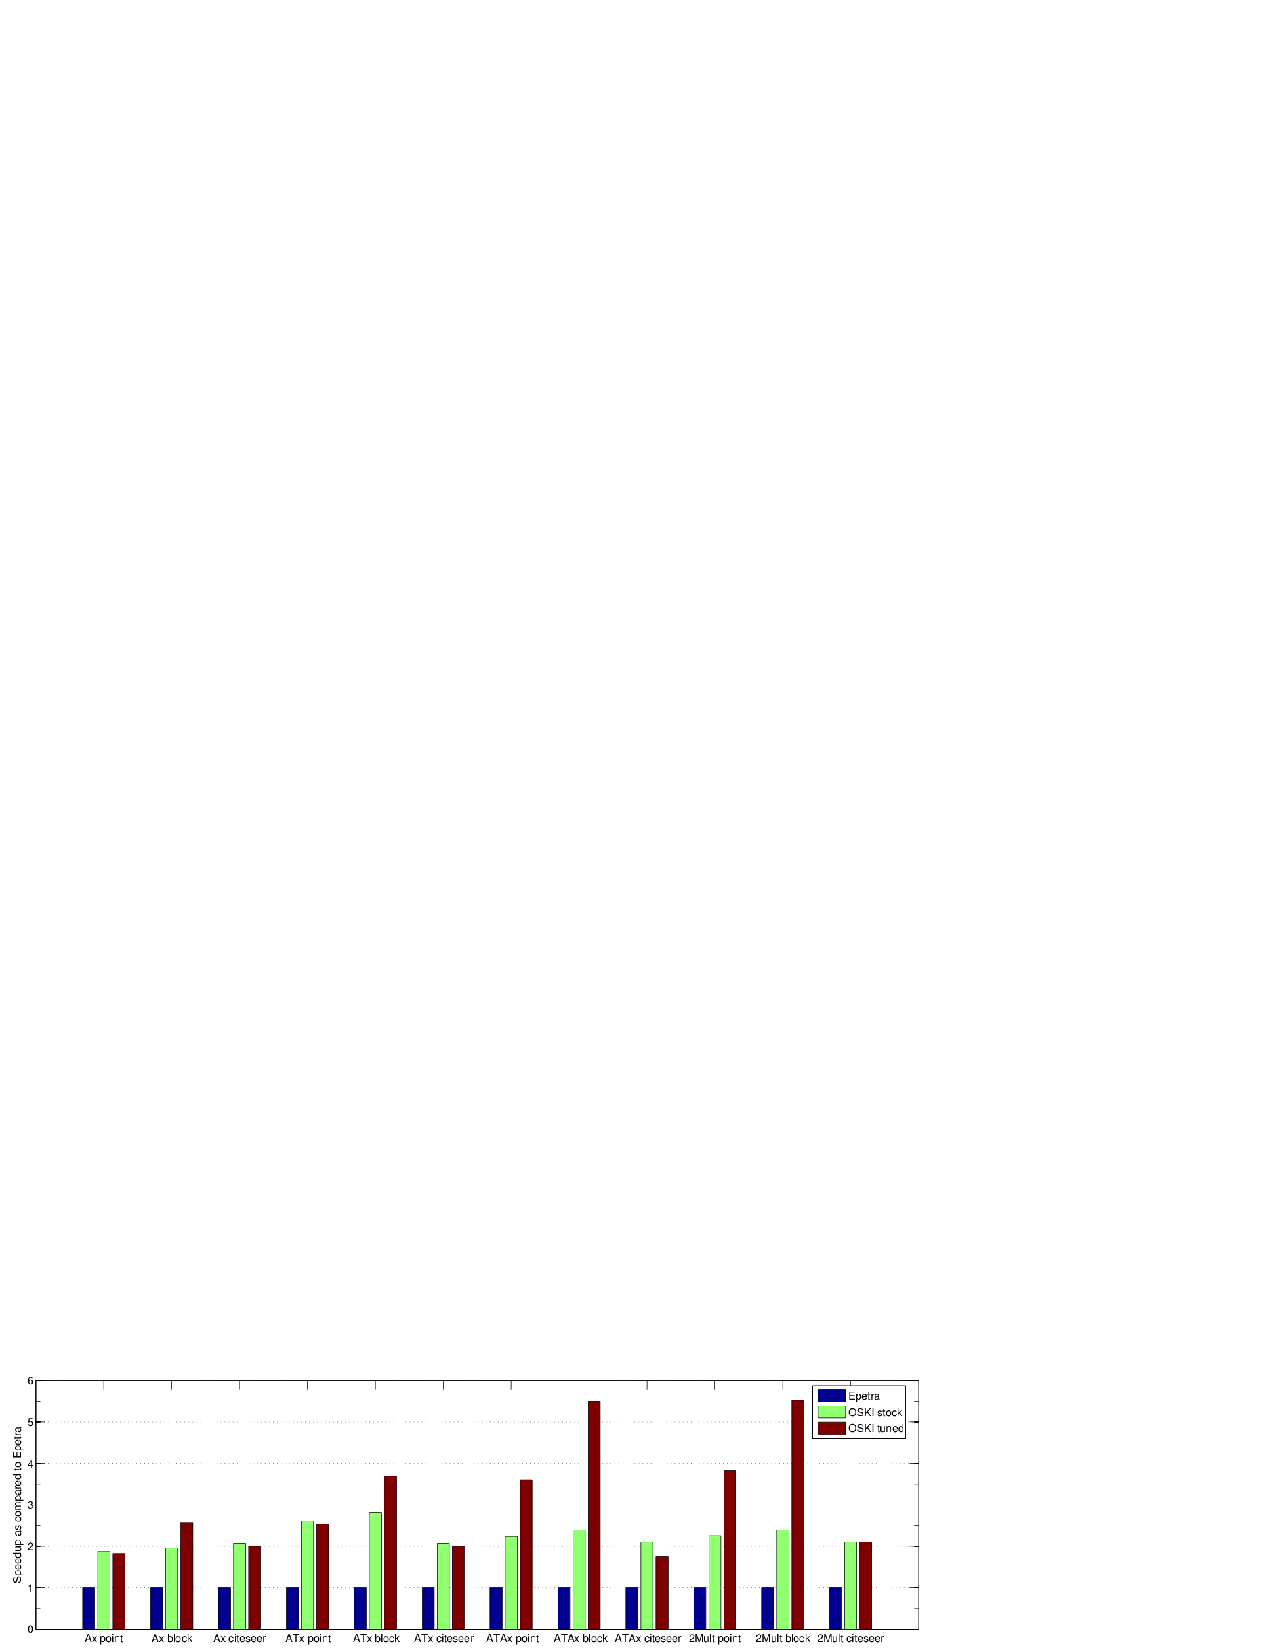
\includegraphics[scale=.8]{./plots/c3serial.pdf}
\caption{Relative performance of Epetra and OSKI in serial on Clovertown.}
\label{IK:fig:C3serial}
\end{center}
\end{figure}
%
\begin{table}[htbp]
\begin{center}
\begin{tabular}{|l|l|l|l|l|}
\hline
Machine & $Ax$ & $A^Tx$ & $A^TA$ & 2Mult \\
\hline
Clovertown & 220/227/55 & 150/154/43 & 178/183/48 & 178/184/48 \\
%barcelona & & & & \\
Niagara & 58.3/69.9/20.7 & 56/66.4/20.3 & 57.1/68.1/20.5 & 57.1/68.1/20.5 \\
\hline
\end{tabular}
\caption{Epetra serial routine speeds in Mflops.  Results are in the form point/block/Citeseer.}
\label{IK:fig:serialnums}
\end{center}
\end{table}

On the Clovertown, OSKI produced large speedups over Epetra for all matrices in serial,
as shown in Figure \ref{IK:fig:C3serial}.
The stock kernels demonstrated speedups of $1.8$ to $2.8$.  Tuning improved the block matrices by about one third
when compared to the stock kernels. The composed algorithms demonstrated even more significant speedups of up to
5.5, when composing and blocking were combined.
Tuning did not improve the runtime of point matrices, except when a composed
kernel was used.  In the
case of the Citeseer matrix, a composed kernel resulted in either no performance gain or performance
degradation.

%\begin{figure}[htbp]
%\begin{center}
%\includegraphics{./plots/barcelonaserial.pdf}
%\caption{Serial results on Barcelona}
%\label{IK:fig:barcelonaserial}
%\end{center}
%\end{figure}

%Barcelona text here when numbers exist.

\begin{figure}[htbp]
\begin{center}
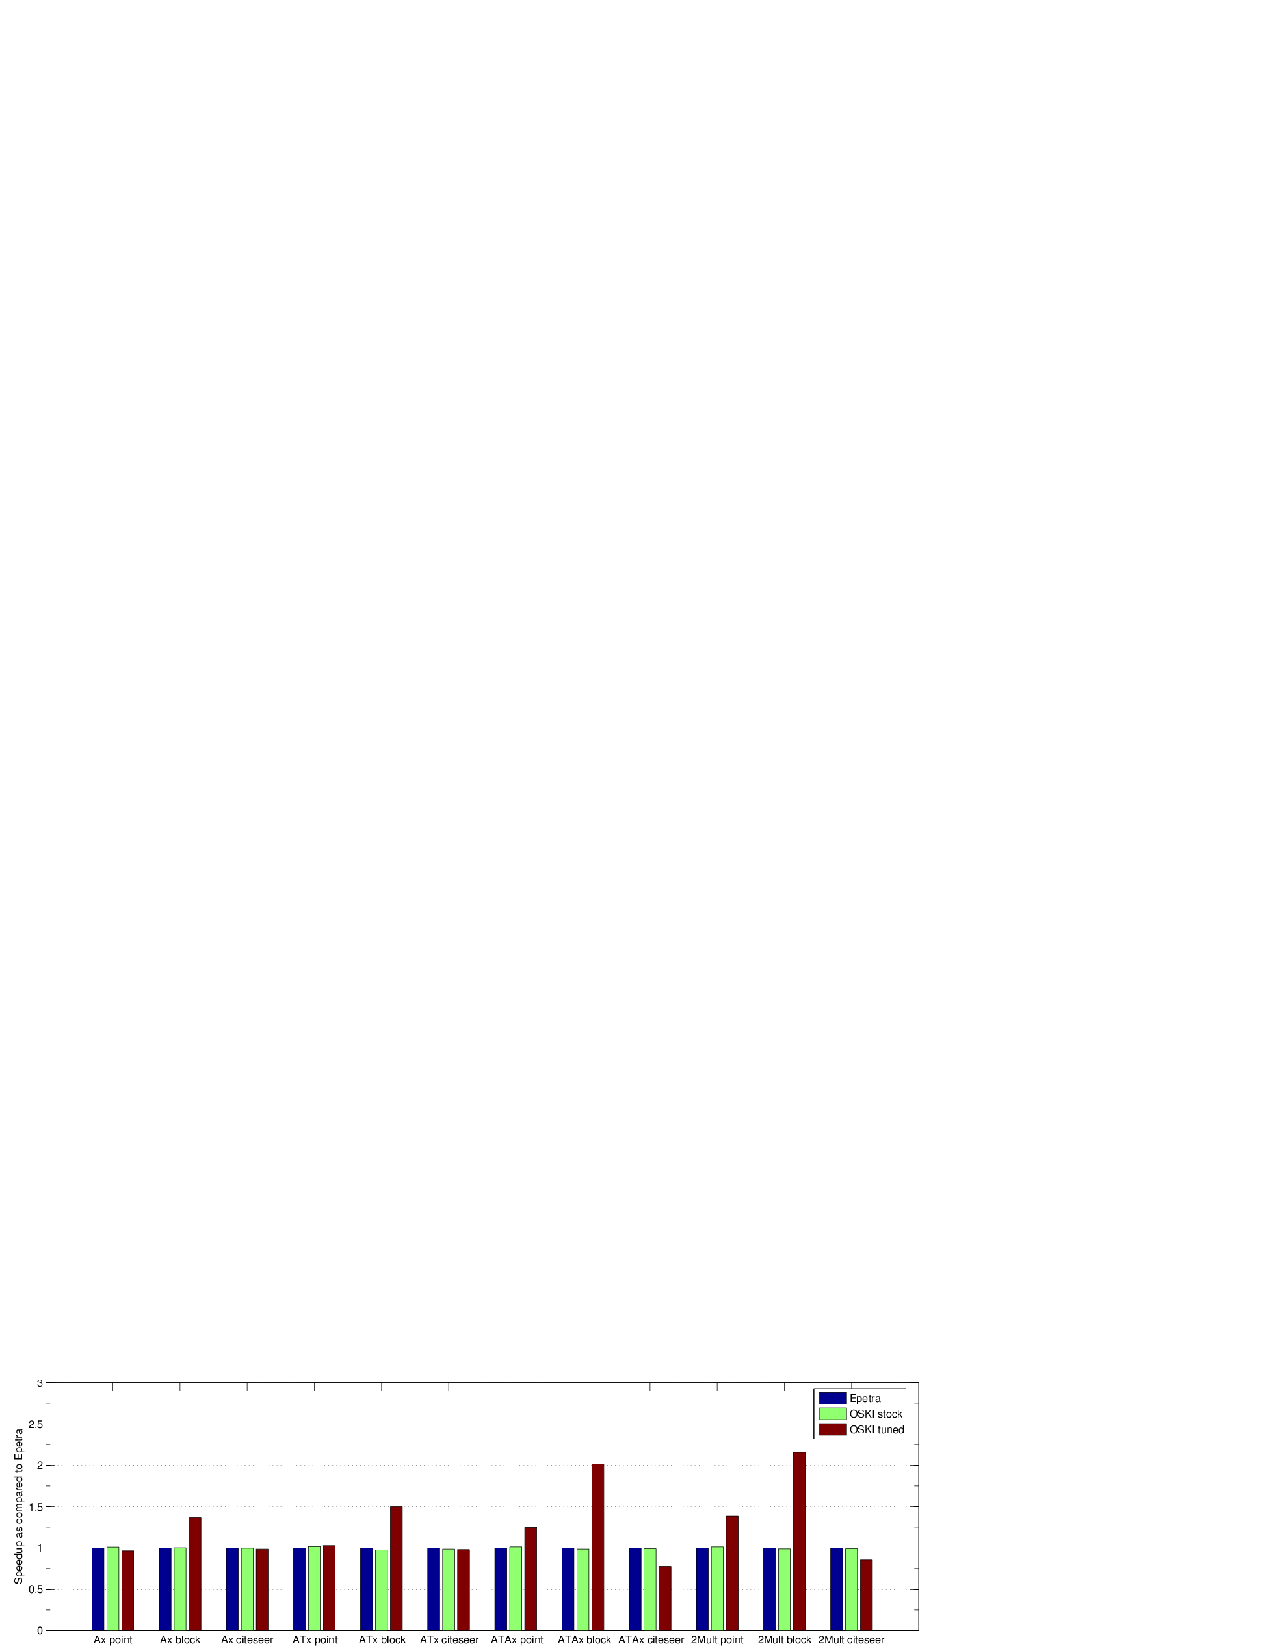
\includegraphics[scale=.8]{./plots/hypnotoadserial.pdf}
\caption{Relative performance of Epetra and OSKI in serial on Niagara.}
\label{IK:fig:hypnotoadserial}
\end{center}
\end{figure}

Figure \ref{IK:fig:hypnotoadserial} shows that
on the Niagara, the stock OSKI and Epetra kernels had roughly the same performance
Tuning for point matrices once again resulted in either no gains or
slight losses. Tuning for block matrices resulted in a one third to one half gain in speed.  Again,
composing increased the speed of all kernels significantly, except for the Citeseer matrix, for which the
OSKI kernels where actually slower.

As expected, the serial tests show that the tuning of point matrices is counterproductive,
except when needed to use composed kernels.
However, tuning of block matrices results in significant speedups through the reduction of indirect addressing.  For the
pseudo random Citeseer matrix, tuning is never beneficial.  This is probably due to either lack of cache-blocking in the composed kernels
 and/or more random access, which create a greater number of cache misses.
% by increasing reuse distances between reads of individual vector elements.
For structured matrices, composing results in a 25\% to 60\% gain over the faster of the stock and tuned kernels.

Even if the tuning gains shown above are large, the amount of time it takes to tune a matrix at runtime is important in determining whether
tuning will result in performance gains.  Tables \ref{IK:fig:tuningcostspoint}, \ref{IK:fig:tuningcostsblock}
and \ref{IK:fig:tuningcostsciteseer} show the cost of tuning and the number of matrix-vector calls needed to amortize that cost for the point, block, and Citeseer matrices, respectively.
 The tuning and retuning costs are expressed in terms of
the number of matrix-vector multiplies that could be performed in the time it takes to tune.
{\it Tuning cost} is the amount of time it takes to tune a matrix the first time, and includes
time to analyze the matrix to determine what optimizations are beneficial.
{\it Retuning cost} is the amount of time it takes to tune the matrix if the optimizations
to be performed are already known.  All comparisons are to the faster of the Epetra and OSKI matrix-vector
multiplies.  The amortize columns show the number of calls to the tuned kernel needed to realize
tuning gains.  When N/A is listed in an amortize column, it is never better to tune
because the tuned kernels are no faster than the untuned kernels.
We note that the tuning cost depends only on the matrix structure, not on the matrix kernel to be
performed.
%
\begin{table}[htbp]
\centering
\begin{tabular}{|l|l|l|l|l|}
\hline
Machine & Tune/Retune & Amortize & Amortize & Amortize \\
 & & $Ax$/Retune & $A^TA$/Retune & 2Mult/Retune \\
\hline
Clovertown & 37.6 / 20.1 & N/A & 48 / 26 & 45 / 24 \\
%Barcelona & & & & \\
Niagara & 22.1 / 12.7 & N/A & 56 / 33 & 40 / 24 \\
\hline
\end{tabular}
\caption{OSKI tuning costs for point matrix.  Cost is equivalent number of matrix-vector multiplications.} \label{IK:fig:tuningcostspoint}
\end{table}

\begin{table}[htbp]
\begin{center}
\begin{tabular}{|l|l|l|l|l|}
\hline
Machine & Tune/Retune & Amortize & Amortize & Amortize \\
 & & $Ax$/Retune & $A^TA$/Retune & 2Mult/Retune \\
\hline
Clovertown & 31.1 / 17.7 & 131 / 75  & 27 / 16 &  28 / 16  \\
%Barcelona & & & & \\
Niagara & 22.5 / 14.1 & 86 / 54 & 22 / 14  & 21 / 13 \\
\hline
\end{tabular}
\caption{OSKI tuning costs for block matrix. Cost is equivalent number of matrix-vector multiplications.}
\label{IK:fig:tuningcostsblock}
\end{center}
\end{table}


\begin{table}[htbp]
\begin{center}
\begin{tabular}{|l|l|l|l|l|}
\hline
Machine & Tune/Retune & Amortize & Amortize & Amortize \\
 & & $Ax$/Retune & $A^TA$/Retune & 2Mult/Retune \\
\hline
Clovertown & 14.5 / 6.7 & N/A & N/A & N/A \\
%Barcelona & & & & \\
Niagara & 11.5 / 5.2 & N/A & N/A & N/A \\
\hline
\end{tabular}
\caption{OSKI tuning costs for Citeseer matrix. Cost is equivalent number of matrix-vector multiplications.}
\label{IK:fig:tuningcostsciteseer}
\end{center}
\end{table}

In many cases, the tuned OSKI kernels are much more efficient than the Epetra and
OSKI stock kernels.
However, the data structure rearrangement required to create an OSKI
kernel is non-trivial. The cost of tunings ranges from 11.5 to 37.6 equivalent matrix-vector multiplies.
It can require as many as 131 subsequent kernel applications to recoup the cost of initial tuning.
However, re-tuning costs are usually slightly over half the cost
of the initial tuning, so saving transformations for later use could be profitable.  Block
matrices require the smallest number of calls to recover tuning costs, and when combined with
composed kernels, this number drops even more.
For point matrices tuning the matrix-vector
multiply is never profitable, but the tuning of composed kernels can be profitable
for structured matrices.

While serial performance is important to application performance, most scientific simulations are
run on parallel machines.  The first level of parallelism is within a single node,
which typically contains one or two multicore processors.  To test the scalability of our
implementation of OSKI, within Epetra, we ran tests on each matrix on 1 to 8 cores of each machine
and also on 1 to 8 threads per core on the Niagara.

\begin{figure}[htbp]
\centering
\subfigure[Clovertown]{
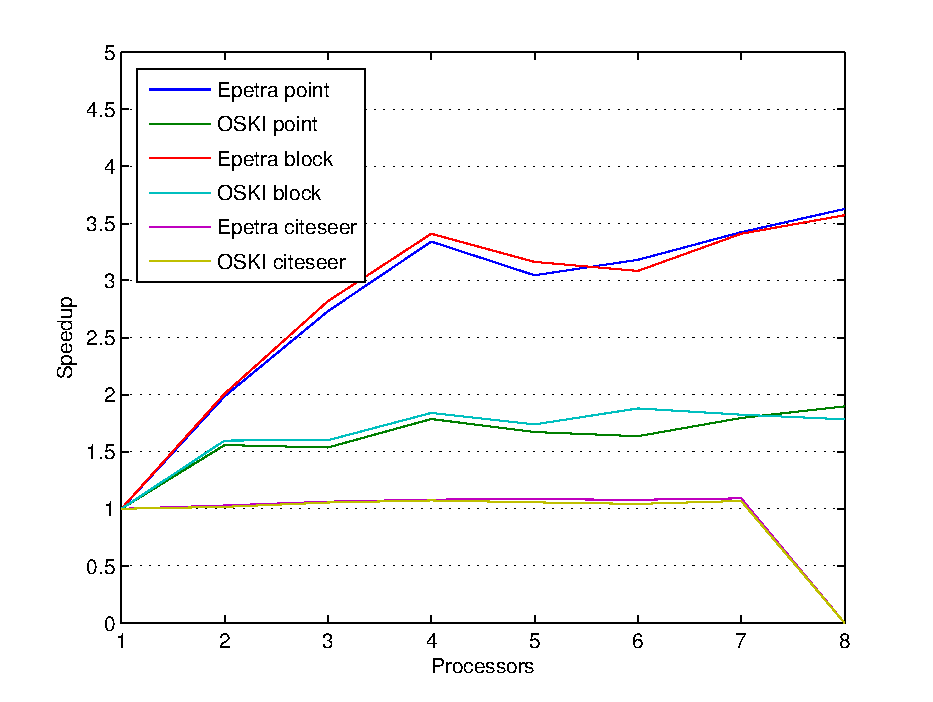
\includegraphics[scale=.39]{./plots/c3scale.pdf}
\label{IK:fig:c3strong}
}
\subfigure[Niagara]{
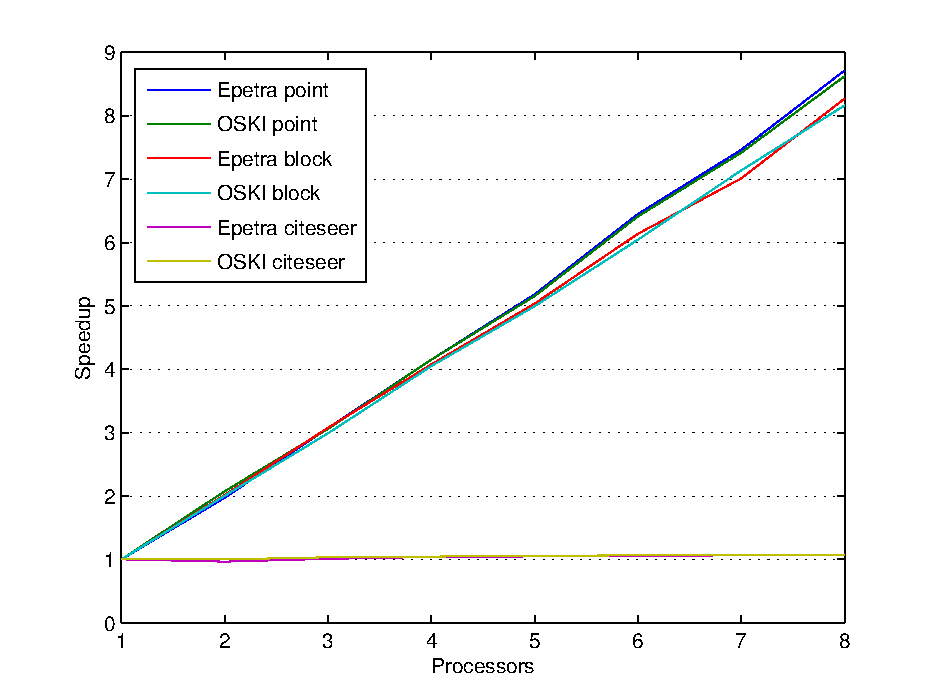
\includegraphics[scale=.39]{./plots/hypnotoadscale.pdf}
\label{IK:fig:hypstrong}
}
\subfigure[Niagara multi-threaded]{
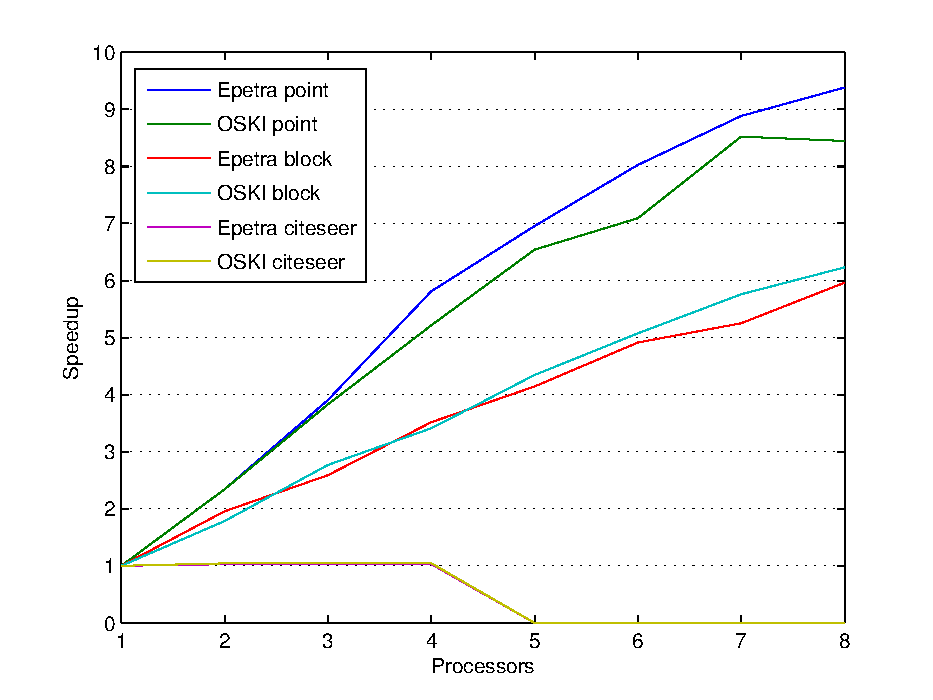
\includegraphics[scale=.39]{./plots/hypnotoadscalebig.pdf}
\label{IK:fig:hypstrongthread}
}
%\caption{Strong scaling results for Clovertown and Niagara processors on top, and Niagara thread scalability on bottom.}
\caption{OSKI matrix-vector multiply strong scaling results.}
\label{IK:fig:strongscale}
\end{figure}

Figures \ref{IK:fig:c3strong}-\ref{IK:fig:hypstrongthread} show the strong scaling of the matrix-vector
kernel for each matrix.  Figure \ref{IK:fig:c3strong}
shows that on the Clovertown that Epetra has better scaling than OSKI. Table
\ref{IK:fig:parrallelnums} shows, however, that the overall performance of OSKI is either comparable or
better to that of Epetra.
The better scaling for Epetra comes from its slower performance in the single processor case, which allows
for more improvement within a limited memory bandwidth situation.
% When most of the matrix fits in cache performance improves faster than
%the number of processors due to increased processing power and decreased memory cost.
For the point matrix, both Epetra and OSKI improve significantly
until each is running at about 735 Mflops on 4 cores.
At this point,  the calculations likely become memory bandwidth limited.
With added processing power, the speeds then improve to slightly under 800 Mflops.
The block matrix results show a similar pattern, with the OSKI block matrix remaining more efficient throughout.
The Citeseer matrix does not scale most likely due to the large amounts of data it needs to exchange, because its
unstructured.  Also it could not be run on 8 processors due to an increasing memory footprint, perhaps due to exchanged data.


\begin{table}[htbp]
\begin{center}
\begin{tabular}{|l|l|l|l|}
\hline
machine & point & block & Citeseer \\
 & Epetra/OSKI & Epetra/OSKI & Epetra/OSKI \\
\hline
Clovertown &  798/782 & 810/1099 & 59.6/122  \\
%barcelona & & & \\
Niagara 1 thread/core & 508/507 & 578/778 & 22.3/22.0\\
Niagara multiple threads/core & 4767/4321 & 3447/4847 & 23.2/23.2 \\
\hline
\end{tabular}
\caption{Epetra and OSKI maximum parallel matrix vector multiply speeds in Mflops.}
\label{IK:fig:parrallelnums}
\end{center}
\end{table}


Figure \ref{IK:fig:hypstrong} shows that on the Niagara both the point and block matrix algorithms scale linearly with the number
of cores.  Essentially, there is enough memory bandwidth to feed each core.  As seen in Figure \ref{IK:fig:hypstrongthread},
 adding more threads per core to the calculating power leads to approximately linear speedup for all matrices.
This begins to tail off at 5 threads for block matrices, and 7 threads for point matrices.  The Citeseer matrix once
again does not scale and becomes too large to run above 32 threads.

Scalability also matters when a matrix is being tuned.  Figures
\ref{IK:fig:c3tuningScal}-\ref{IK:fig:niagthreadtuningScal} show
how well each matrix scales on each machine in terms of tuning cost.  Scaling is usually
linear or slightly better with the number of processors.  This result is expected as tuning is
a local computation with no communication between processors.  As seen in Figure \ref{IK:fig:niagthreadtuningScal},
increasing
the number of threads per Niagara processor initially leads to improved performance, before dropping off at 6
or  more threads per processor.
The dropoff is most likely due to threads competing for processor resources.  Results for the Citeseer matrix were
not shown, as OSKI does not tune its matrix-vector multiply kernel for the Citeseer matrix.  Finally, note
that the retune function demonstrates better scaling than the same tune function in all cases.

\begin{figure}[htbp]
\begin{center}
\subfigure[Clovertown]{
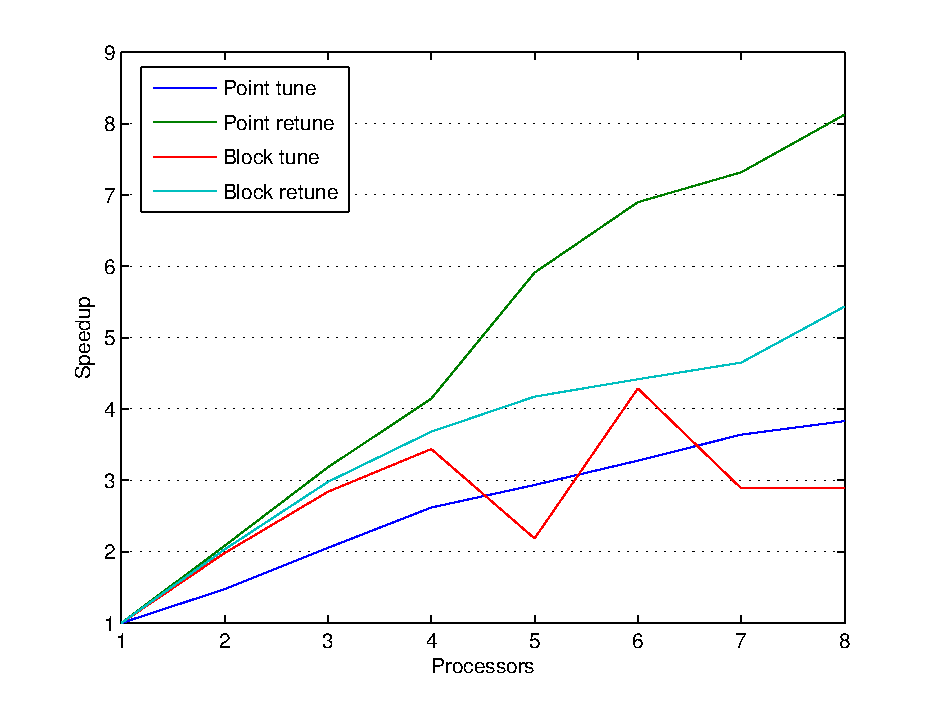
\includegraphics[scale=.4]{./plots/c3tune.pdf}\label{IK:fig:c3tuningScal}}
\subfigure[Niagara single-threaded]{
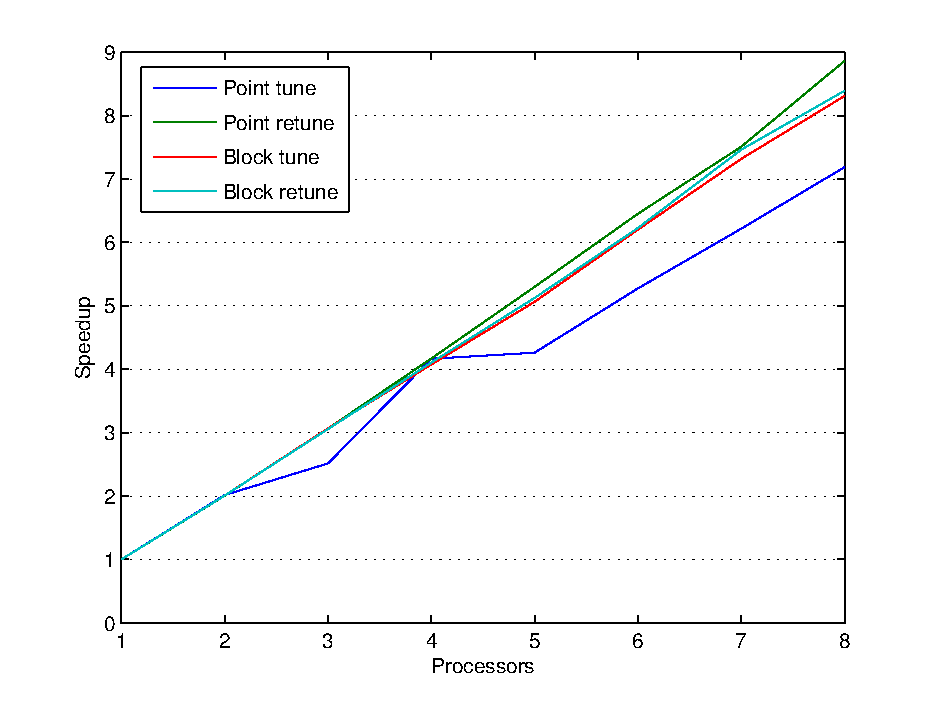
\includegraphics[scale=.4]{./plots/hypnotoadtune.pdf}\label{IK:fig:niagtuningScal}}
\subfigure[Niagara multi-threaded]{
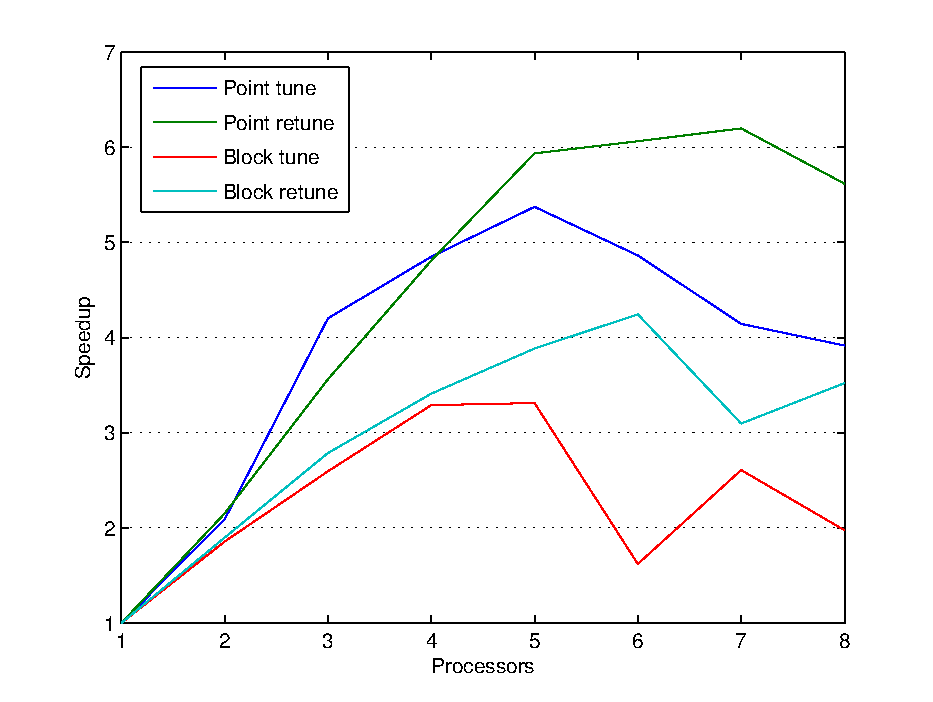
\includegraphics[scale=.4]{./plots/hypnotoadtunebig.pdf}\label{IK:fig:niagthreadtuningScal}}
\caption{Scalability of OSKI tuning.}
% scalability Clovertown and Niagara processor scalability on top and Niagara thread scalability on bottom.}
\label{IK:fig:tuningscale}
\end{center}
\end{figure}

In addition to strong scaling tests, we also ran a weak scaling test on the Niagara.  We used the block
matrix from the 8 thread test case in Table \ref{IK:fig:serialmats}.  Tests were run on 1, 8, 27 and 64 threads.
Results are shown in Figures \ref{IK:fig:weakmatvec}-\ref{IK:fig:weaktune}.  As seen in Figure \ref{IK:fig:weakmatvec}, the OSKI tuned and untuned  matrix-vector
multiplies both scale similarly to Epetra's matrix-vector multiply.  Figure \ref{IK:fig:weakcomposed}, shows that the tuned
composed kernels do not scale well.  The same result was seen for the untuned composed kernels.  For these operations
to be possible there is extra data copying in the wrapping of the serial kernels, which could be the problem.  There could also be
inefficiencies in the code in other places or resource contention on the processor.
%, however, it is not known at this time why this issue is occurring.
Figure \ref{IK:fig:weaktune} shows that re-tuning scales better than tuning as
the problem size grows.

\begin{figure}[htbp]
\begin{center}
\subfigure[MatVec]{
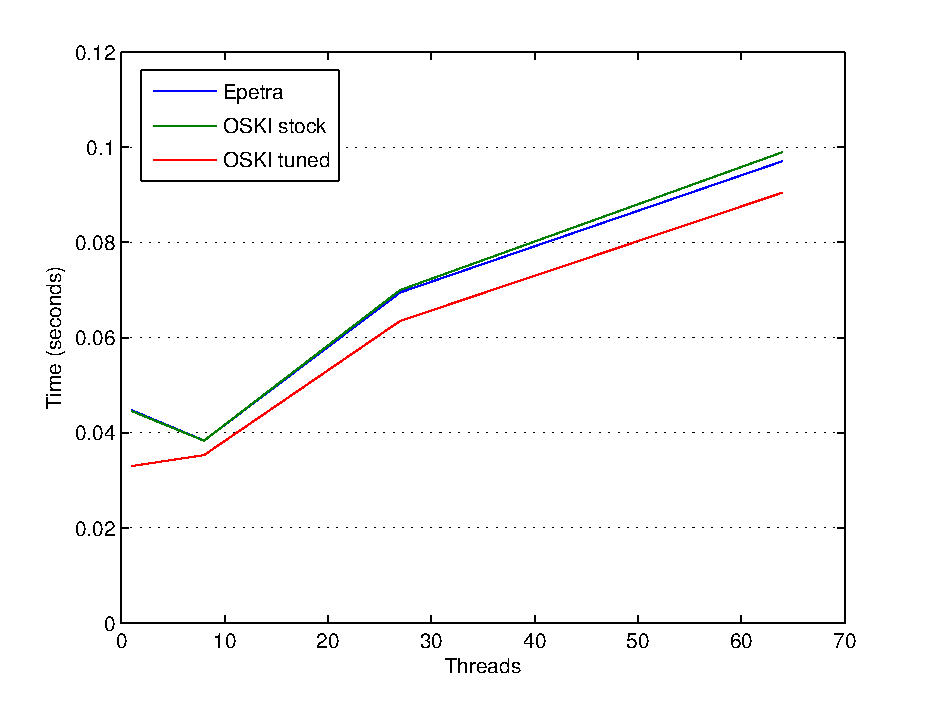
\includegraphics[scale=.4]{./plots/weakmatvec.pdf}\label{IK:fig:weakmatvec}}
\subfigure[Composed]{
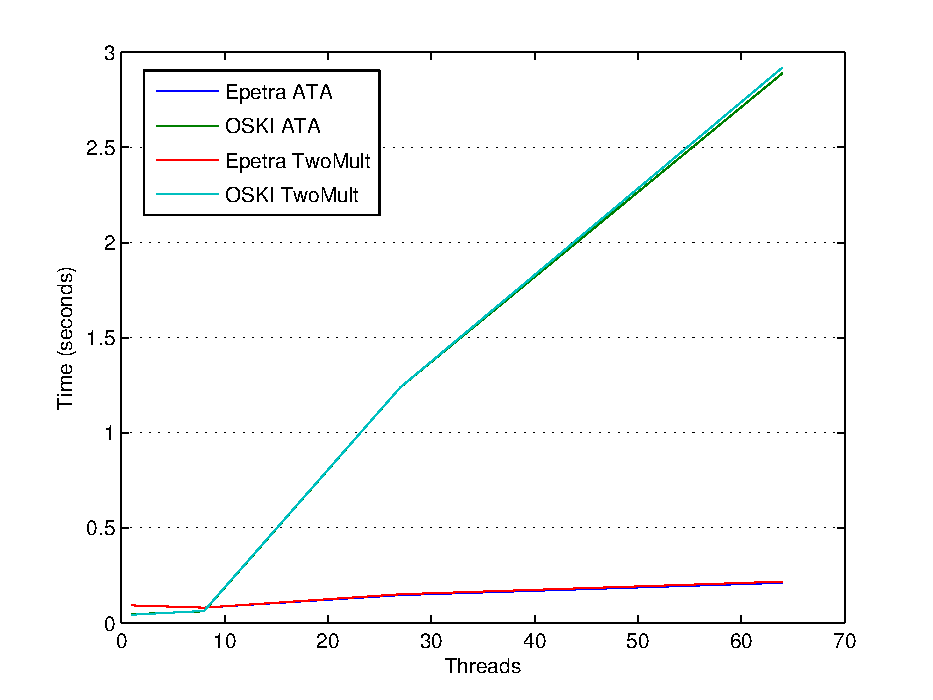
\includegraphics[scale=.4]{./plots/weakcomposed.pdf}\label{IK:fig:weakcomposed}}
\subfigure[Tuning]{
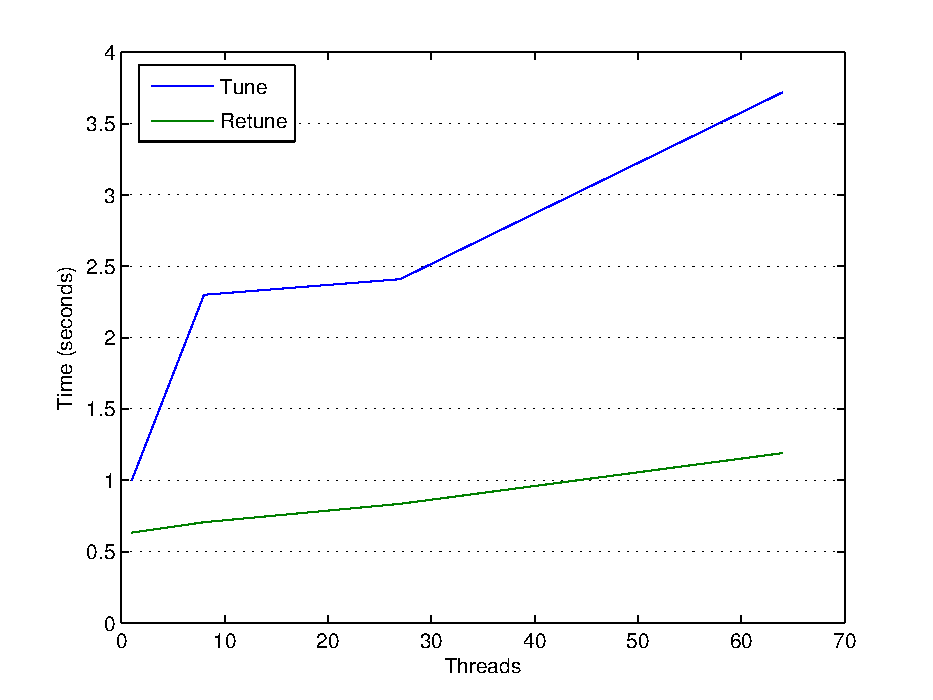
\includegraphics[scale=.4]{./plots/weaktune.pdf}\label{IK:fig:weaktune}}
\caption{Weak scalability of OSKI on Niagara}
% scalability Clovertown and Niagara processor scalability on top and Niagara thread scalability on bottom.}
\label{IK:fig:weakscale}
\end{center}
\end{figure}

%Then maybe a weak scaling numbers that need to be run.
%
%Finally cluster numbers if run.


\section{Conclusions} \label{IK:sec:conclu}
Overall, OSKI can produce large speedups in sparse matrix computational kernels.  This is especially
true
when the matrix is block structured or multiple multiplications are performed
using the same matrix.  In some cases it can also produce large gains for matrix-vector
multiplies involving only a single matrix.  However, OSKI is still
missing some features, such as a multi-vector kernel and the ability to tune
matrices to make them symmetric. Both could produce large runtime gains.  Our Epetra/OSKI
interface has stubs to allow the use of these missing features as soon as they become available in
OSKI.  Our experiments show that Sandia applications that make heavy use certain sparse matrix kernels
can benefit from the current version of OSKI.  As new OSKI features
become available, its potential impact on other Sandia applications should increase.


\section{Future Work} \label{IK:sec:future}
%A future developer or person performing analysis of a new version of OSKI would want to start
%at the following places.
For the current (1.0.1h) version of OSKI, a developer may want to implement the solve function
and run more weak scalability or other parallel tests to determine why the composed kernels do not scale
well.
For a newer version of OSKI,
a developer may want to test any new tuning features,
the matrix power kernel, as well as any other new functions.
Finally, we recommend  any new version of OSKI be tested
on the Barcelona and Xeon chips, as we were never able to successfully install OSKI on these
architectures.
The Barcelona is of particular interest, as it is the processor found in the center section of Red Storm.
%Before the final submission of the paper we hope to have run tests on the quad-core AMD Barcelona chip,
%have parallel results for the citeseer matrix, have run a larger block matrix,
%run weak scaling tests, and a test on a cluster.


\section{Acknowledgments} \label{IK:sec:acknowledgments}
Many people have helped develop \ifpacktwo{}, and we would like to acknowledge
their contributions here: Ross Bartlett, Tom Benson, Erik Boman, Joshua Booth,
Julian Cortial, Kevin Deweese, Jeremie Gaidamour, Paul Lin, Travis Fisher, Sarah
Osborn, Eric Phipps, and Paul Tsuji. Finally, Alan Williams did the original
port from \ifpack{} and was the original lead developer of \ifpacktwo{}.


\bibliographystyle{siam}
% Edit the line below to be your first and last names.
\bibliography{EpetraOski}

% Edit FirstnameLastname below to be your first and last names, but leave the line commented out.
% This line will help me merge bibliographies for the proceedings.
%\input{IanKarlin/IanKarlin.bbl}

\end{document}
